\section*{\color{olive}Ejercicio 1: Medici\'on de curvas caracter\'isticas de diodos}

A continuaci\'on se presentan los circuitos empleados para medir la curva caracter\'istica (corriente en funci\'on de la tensi\'on) de un diodo rectificador, de un diodo zener y de un LED. En los tres casos se coloca una resistencia en serie de $1k\Omega$, con la finaldidad de limitar la corriente que circula por cada uno de ellos.

\begin{figure}[h!]
 \begin{center}
    \begin{circuitikz}
    \draw (0,3)
	%(0,0) node[ground] {}
      to[V,v=$V_{cc}$] (0,0) % The voltage source
	(0,3) to[Do] (2,3)
%  (0,3) to[short] (1,3) node[fulldiodeshape]{} 
%	(1,3) to[short] (2,3)
      to[R=$R_1$] (2,0) % The resistor
	to[short] (2,0)
	to[short] (1,0) node[ground]{}
	(1,0) to[short] (0,0);

    \draw (6,3)
	%(0,0) node[ground] {}
      to[V,v=$V_{cc}$] (6,0) % The voltage source
	(6,3) to[zDo] (8,3)
%  (0,3) to[short] (1,3) node[fulldiodeshape]{} 
%	(1,3) to[short] (2,3)
      to[R=$R_1$] (8,0) % The resistor
	to[short] (8,0)
	to[short] (7,0) node[ground]{}
	(7,0) to[short] (6,0);

    \draw (12,3)
	%(0,0) node[ground] {}
      to[V,v=$V_{cc}$] (12,0) % The voltage source
	(12,3) to[leDo] (14,3)
%  (0,3) to[short] (1,3) node[fulldiodeshape]{} 
%	(1,3) to[short] (2,3)
      to[R=$R_1$] (14,0) % The resistor
	to[short] (14,0)
	to[short] (13,0) node[ground]{}
	(14,0) to[short] (12,0);
    \end{circuitikz}

    \caption{Circuitos empleados para medir la curva caracter\'istica de un diodo rectificador, de un diodo zener y de un LED; respectivamente.}
\end{center}
\end{figure}

%%% diodo rectificador
\subsection*{\color{orange}Diodo rectificador}

A continuaci\'on se presentan los gr\'aficos obtenidos de la corriente vs. tensi\'on para el caso del diodo rectificador 1N4148. En la figura \ref{med1a} se puede ver la simulaci\'on realizada. En la figura \ref{med1b} se puede ver, a la izquierda, los datos obtenidos del osciloscopio mediante un CSV y a la derecha el gr\'afico de la corriente en funci\'on de la tensi\'on a partir de las tensiones medidas con osciloscopio y del valor conocido de la resistencia.

\begin{figure}[H]
\centering
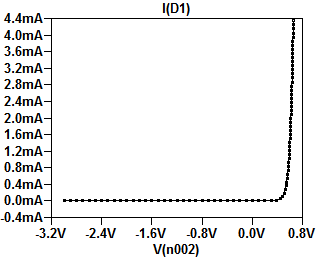
\includegraphics[scale=0.8]{../EJ1/DiodoRectificador/corrienteDiodo1}
\caption{Simulaci\'on corriente vs. tensi\'on del diodo rectificador.}
\label{med1a}
\end{figure}

\begin{figure}[H]
\centering
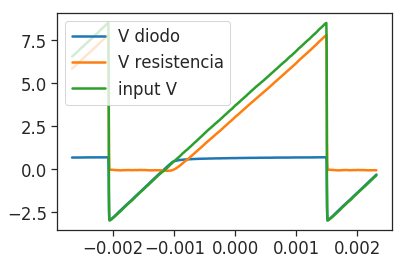
\includegraphics[scale=0.5]{../EJ1/DiodoRectificador/datosOsciloscopio}
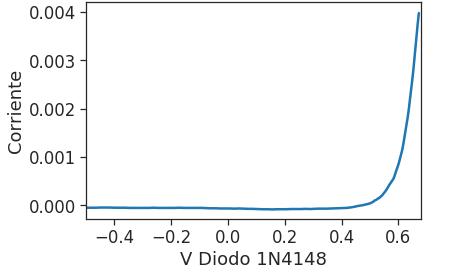
\includegraphics[scale=0.5]{../EJ1/DiodoRectificador/diodoRectMedido}
\caption{Medici\'on de la corriente vs. tensi\'on del diodo rectificador: Datos obtenidos y datos procesados; respectivamente.}
\label{med1b}
\end{figure}

\begin{figure}[H]
\centering
\includegraphics[scale=0.8]{../EJ1/DiodoRectificador/corrienteDiodoDatasheet}
\caption{Corriente vs. tensi\'on del diodo rectificador obtenida de la hoja de datos.}
\label{med1c}
\end{figure}

De la figura \ref{med1c} obtenida de la hoja de datos del diodo 1N4148, a nuestro caso corresponde la curva (2).

Se puede ver que la curva caracter\'istica del diodo obtenida con la medici\'on es muy similar tanto a la simulaci\'on, como a la curva de la hoja de datos de dicho componente.

%%% diodo zener
\subsection*{\color{orange}Diodo zener}

A continuaci\'on se presenta la simulaci\'on del gr\'afico de la corriente en funci\'on de la tensi\'on correspondiente al diodo zener en la figura \ref{med2a}, y en la figura \ref{med2b} el gr\'afico obtenido a partir de las mediciones del osciloscopio. Para obtener este \'ultimo se procedi\'o de la misma manera que para obtener el correspondiente al diodo rectificador.

\begin{figure}[H]
\centering
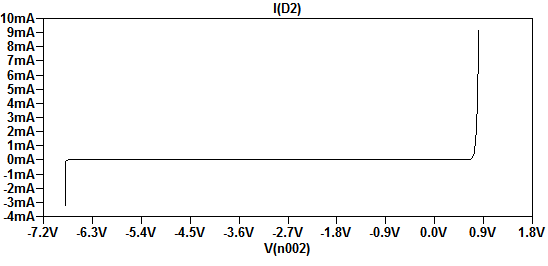
\includegraphics[scale=0.8]{../EJ1/DiodoZener/simulacionZener}
\caption{Simulaci\'on corriente vs. tensi\'on del diodo zener.}
\label{med2a}
\end{figure}

\begin{figure}[H]
\centering
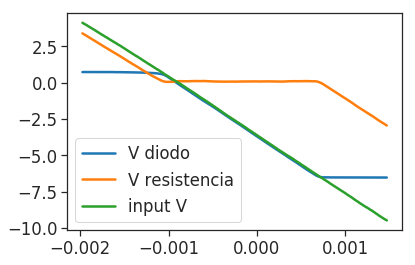
\includegraphics[scale=0.5]{../EJ1/DiodoZener/datosOsciloscopioZener}
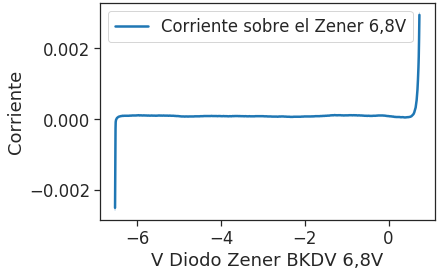
\includegraphics[scale=0.5]{../EJ1/DiodoZener/zenerMedido}
\caption{Medici\'on de la corriente vs. tensi\'on del diodo zener: Datos obtenidos y datos procesados; respectivamente.}
\label{med2b}
\end{figure}

%\begin{figure}[!ht]
%\centering
%\includegraphics[scale=0.52]{../EJ1/DiodoZener/corrienteDiodoDatasheet}
%\caption{Corriente vs. tensi\'on del diodo zener obtenida de la hoja de datos.}
%\label{med2c}
%\end{figure}

%%% led
\subsection*{\color{orange}LED}

%\begin{figure}[H]
%\centering
%\includegraphics[scale=0.62]{../EJ1/LED/simulacionLED}
%\caption{Simulaci\'on corriente vs. tensi\'on del LED.}
%\label{med3a}
%\end{figure}

\begin{figure}[H]
\centering
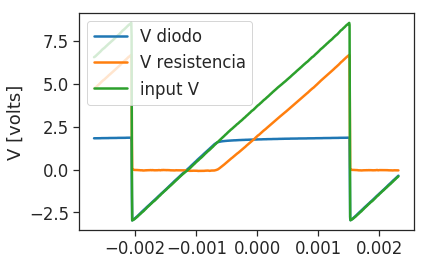
\includegraphics[scale=0.5]{../EJ1/LED/datosOsciloscopioLED}
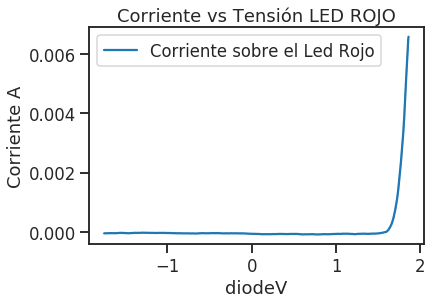
\includegraphics[scale=0.5]{../EJ1/LED/LEDMedido}
\caption{Medici\'on de la corriente vs. tensi\'on del LED: Datos obtenidos y datos procesados; respectivamente.}
\label{med3b}
\end{figure}

\begin{figure}[!ht]
\centering
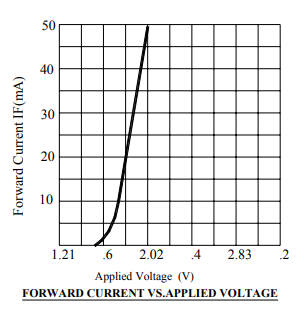
\includegraphics[scale=0.8]{../EJ1/LED/LedDataSheet}
\caption{Corriente vs. tensi\'on del LED obtenida de la hoja de datos.}
\label{med3c}
\end{figure}
